\chapter{二类生物标记物定位问题实验评估}\label{sec:experiments}
\section{前言}
在第\ref{sec:method}章中,本文详细介绍了所提出模型的结构、背后的原理、损失函数等内容。接下来,本文将进行相关实验评估。在本章中,文本将展示本文提出的模型在二类视网膜糖尿病病变数据集和二类模拟皮肤病病变数据集上的相关实验结果,并对其展开分析。首先在\ref{sec:exper_ds_intro}小节中介绍以上两个用于生物标记物定位的数据集,包括数据量、类别数量、生物标记物特点等信息。在\ref{sec:exper_evaluation_metrics}小节中,本文将介绍本章实验所选择的实验评价标准(P-R曲线及其AUC)及其原因。\ref{sec:exper_setting}小节将会介绍本章的实验设置,包括学习率、超参数、数据预处理、训练集/验证集划分等相关信息。从\ref{sec:bin_dr_ds_experiment}小节开始,本章将展示本文提出的模型在以上两个数据集上的实验结果,包括与CAM和Grad-CAM进行的对比实验和针对本文提出的模型的消融实验。具体来说,在\ref{sec:bin_dr_ds_experiment}小节和\ref{sec:bin_simulated_ds_experiment}小节中,本章将本文提出的方法和CAM以及Grad-CAM进行在两个数据集上的对比实验,通过P-R曲线及其AUC来比较各方法模型的性能表现。在\ref{sec:g_c_g_d_g_d_c_comparsion}小节中,利用二类视网膜糖尿病病变数据集,本章通过分别去掉CNN分类器模块和判别器模块的方式设计消融实验来探究本文提出的模型中的各个子模块所扮演的角色。在\ref{sec:indirect_quantitative_evaluation}小节中,本章基于在理想情况下,将异常图像作为输入,经过编码器-解码器之后的输出图像将极少甚至不再包含生物标记物,那么这些输出图像将会被分类器分类为正常的设想,通过对比二类视网膜糖尿病病变数据集和经过编码器-解码器的该数据集的分类情况来间接定量评估本文提出的模型的性能表现。\ref{sec:hyper_paras}小节将设置不同的超参数组合,来探究本文提出的模型的鲁棒性。在\ref{sec:dis_arch}小节中,本章将探究不同的判别器网络结构下,本文提出的模型的性能表现,以期读者能对判别器模块更为深刻的认识。接下来,本章将进行以上内容的具体阐述。
\section{数据集介绍}\label{sec:exper_ds_intro}
在本章中,本文将详细介绍本文提出的模型在处理二类问题时的性能表现。在\ref{sec:usually_ds_intro}小节中,本文介绍了包括眼底病变数据集和黑色素瘤皮肤病病变数据集在内的诸多可用于生物标记物定位任务的常见数据集。考虑到本文的研究内容是生物标记物分布比较分散、生物标记物尺寸大小不一的生物标记物定位任务(黑色素瘤皮肤病病变图像中的异常区域所占比例通常在$1/3$以上且往往没有专门的正常图像),本文将使用包括二类视网膜糖尿病病变数据集(\ref{subsec:bin_dr_ds}小节)和二类模拟皮肤病病变数据集(\ref{subsec:bin_simulated_skin_ds}小节)在内的两个数据集来评估我们提出的模型用于生物标记物定位的表现。因此,在实验评估之前非常有必要先详细介绍以上两个数据集,以便让读者对于本文要解决的问题能有更为清晰的认识与更为明了的理解。下面将进行相关内容的具体叙述。
\subsection{二类视网膜糖尿病病变数据集}\label{subsec:bin_dr_ds}
二类视网膜糖尿病病变数据集是来自Kaggle视网膜糖尿病病变数据集(原始数据集的相关内容介绍请参见\ref{subsec:original_dr_dataset_intro}小节,在此不做赘述),该数据集由从Kaggle视网膜糖尿病病变数据集中选择出来的2,101张包含明确的糖尿病生物标志物的异常图像和2,101张正常图像组成。同时,在预处理阶段,我们先将图像中没有信息的四个黑角去掉;另外,由于眼底图像中的视网膜基本是呈圆形的,故在此基础上,我们还提取了视网膜的边界再根据视网膜边界取其最大内接矩形,从而彻底去掉眼底图像中的不包含任何信息的黑色部分,最后将图像尺寸大小重新调整到$128\times 128$。来自二类视网膜糖尿病病变数据集的部分图像举例如图\ref{subfig:bin_dr_ds_example}所示。另外,可通过比较图\ref{fig:biomarker_localization_example}与图\ref{subfig:bin_dr_ds_example},来对比视网膜糖尿病性病变图像预处理前后的差异。另外,一方面,为了在后续章节中说明本文模型方法的有效性以及增加实验结果的可信度;另外一方面,Kaggle视网膜糖尿病病变数据集本身没有像素级标注而在所有的异常图像中标出所有生物标记物的精确位置又是极其昂贵的,因此,我们随机选出了40张眼底图像并请两位专业眼科医师对其中所有的生物标记物进行了像素级标注,用于后续章节的定量分析。

从图\ref{subfig:bin_dr_ds_example}可以看出,眼底图像中含有丰富的血管,呈现一种随机走向,并且包含非常丰富的毛细血管网,这种充分而又精细的血管纹理细节本身就给图像的重建增加了困难,而图像重建只是本文模型方法中最为基础的一步。我们注意到视网膜糖尿病性病变图像中的血管所在像素位置的梯度明显高于周围像素,为了让编码器-解码器重建图像更为容易,本文使用Sobel梯度算子~\cite{sobel2014history}沿着水平和竖直两个方向的提取图像每个像素的梯度,将其作为L1损失函数的权重。另外,图像之间的背景亮度不易,比如,图\ref{subfig:bin_dr_ds_example}中,第一行第三列图像背景较亮,而第二列第一行图像背景较暗。就生物标记物本身来说,也呈现一种分散、大小不一、不够明显而又难以被察觉的特点,而且还能发现,生物标记物本身的颜色与背景颜色比较相近,比如图\ref{subfig:bin_dr_ds_example}中的第二列第三行和第一列第三行图像,因此这些生物标记物很容易与背景相混淆,这也是在二类视网膜糖尿病病变数据集上完成生物标记物精确定位任务最大的难点。二类视网膜糖尿病性病变图像的这些特点都表明在该数据集上完成生物标记物定位的任务极具挑战性。另外,视网膜糖尿病性病变也是当今导致病人失明的主要原因,说明了该任务的具有较大现实意义和应用潜能。注意,有些生物标记物的边界不仅呈现一种不规则状况,边界还十分模糊,用矩形框圈出生物标记物的位置相对比较容易,但是做出像素级精确标注却比较难,这也是本文只随机选出40张图像做标注的主要原因。

\subsection{二类模拟皮肤病病变数据集}\label{subsec:bin_simulated_skin_ds}
二类模拟皮肤病病变数据集包含带有人工生物标记的皮肤图像。为了生成这个数据集,我们首先从一个皮肤镜图像数据集~\cite{codella2018skin}(原始数据集相关内容介绍可参见\ref{subsec:original_dermatoscope_ds_intro}小节)中提取了$2,920$张图像尺寸大小为$128\times128$的正常图像(实际上是通过滑动窗口方式得到的图像区域块)。为了模拟真实皮肤图像中生物标志物的数量、大小和所在位置的随机变化,我们通过随机参数控制,在每个模拟皮肤图像的一定范围内随机生成这些参数的值。更具体地说,对于每张异常图像,从Image-Net数据集~\cite{deng2009imagenet}中随机选择一到三张图像,并将其调整为尺寸大小为$4\times 4$、$8\times 8$或$16\times 16$的缩略图。再将缩略图嵌入到皮肤图像中,最后将其局部平滑作为人工生物标记。最终,二类模拟皮肤病病变数据集中共有异常图像$1,310$张,正常图像$1,460$张。注意,此数据集中的所有异常图像的人工生物标记物都有像素级的标注。

从图\ref{subfig:bin_simulate_skin_example}中可以看出,二类模拟皮肤病病变数据集中图像之间的背景差异比较大,主要表现在颜色和亮度,比如图中第二行第三列图像背景为红色,较亮,而第一行第二列图像背景则较暗。注意,由于本文对于所有异常图像中的生物标记物都做了局部平滑处理,故此数据集中的生物标记物也显得比较真实,最为明显的特点是其边界比较模糊。再加上引入了生物标记物大小、数量和位置这三个随机变化量,这也大大增加了在此数据集上实现生物标记物的精确定位的难度。与二类视网膜糖尿病病变数据集相比,虽然生物标记物在纹理结构上并没有前者复杂,但是二类模拟皮肤病病变数据集的优势在于拥有所有生物标记物的像素级标注,故可在整个数据集上进行全面的定性分析,来反应出各个模型方法在生物标记物精确定位任务上的性能表现,而二类模拟皮肤病病变数据集本身的模拟生物标记物也比较接近真实,从而保证了从该数据集得出的实验结果的可行性和可靠性,这也是设置该数据集的意义所在。
\begin{figure}[h!]
	\centering
	\begin{subfigure}{0.48\textwidth}
		\centering
		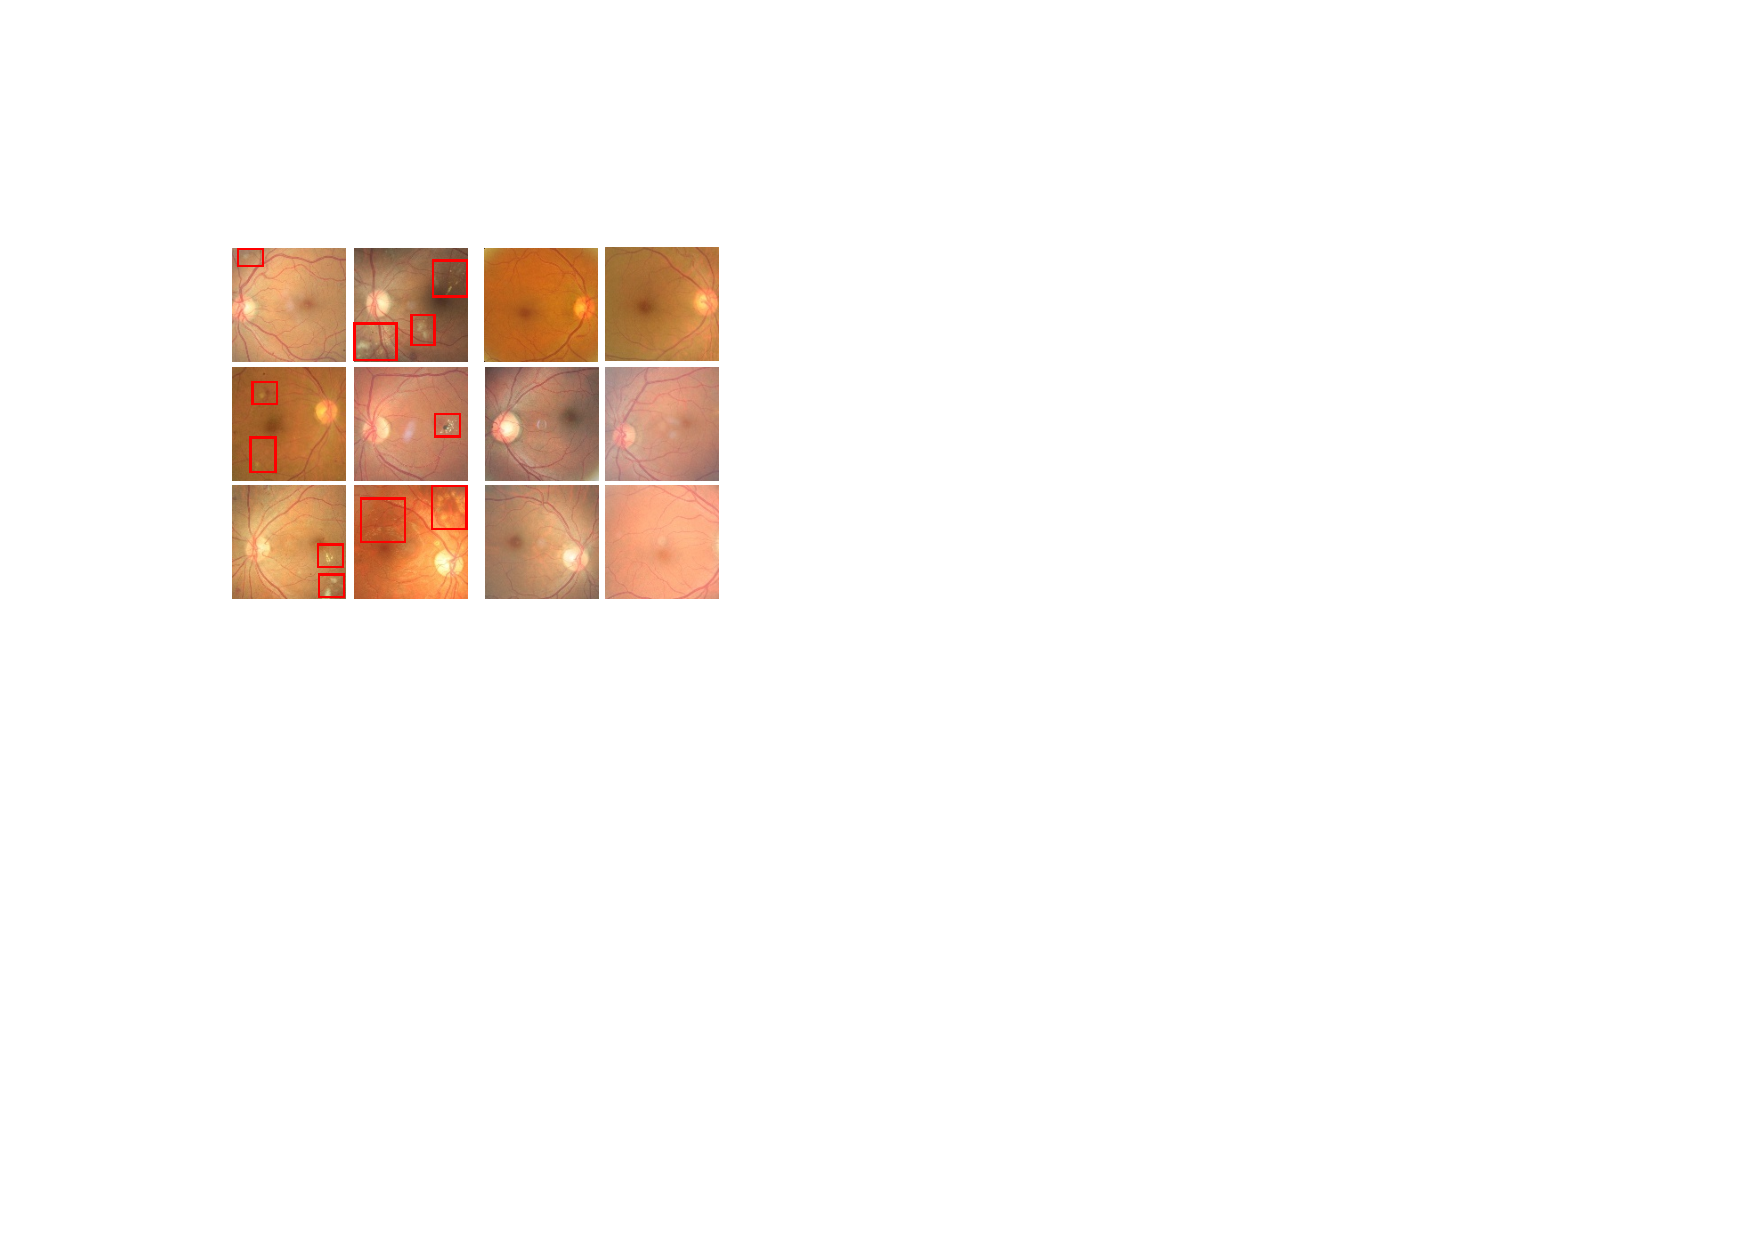
\includegraphics[width=1\textwidth]{figure/bin_dr_ds_example}
		\caption{二类视网膜糖尿病病变数据集部分图像示例。第1、2列是异常图像,第3、4列是正常图像。}
		\label{subfig:bin_dr_ds_example}
	\end{subfigure}
	\quad
	\begin{subfigure}{0.48\textwidth}
		\centering
		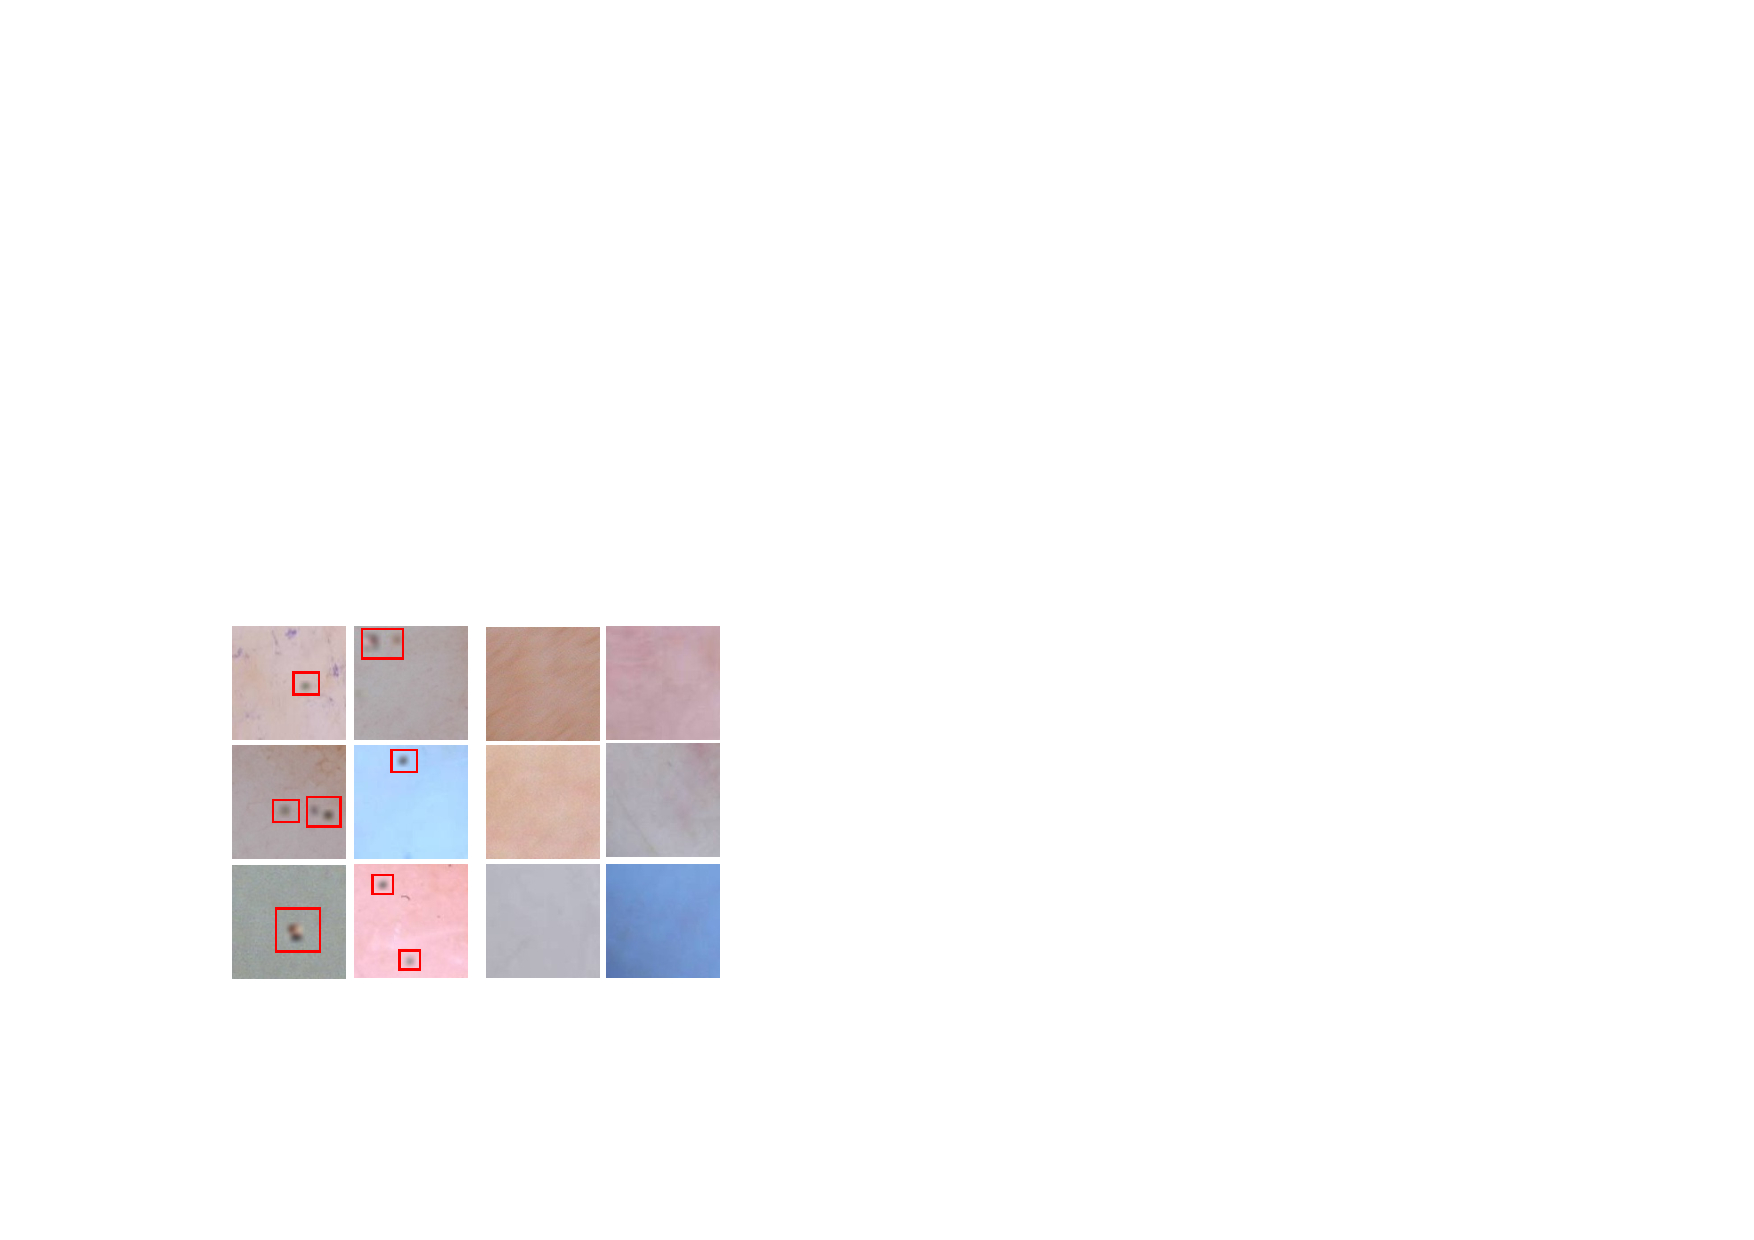
\includegraphics[width=1\textwidth]{figure/bin_simulate_skin_example}
		\caption{二类模拟皮肤病病变数据集部分图像示例。第1、2列是异常图像,第3、4列是正常图像。}
		\label{subfig:bin_simulate_skin_example}
	\end{subfigure}
	\caption{来自二类视网膜糖尿病病变数据集和二类模拟皮肤病病变数据集的部分图像示例。红色矩形框表示框内存在生物标记物或者说框出区域是患病区域。在子图\ref{subfig:bin_dr_ds_example}中,每张图像中明显比周围要亮的圆形区域为视盘,为眼底图像的共有结构,而有些图像视盘在左边,有些视盘在右边,这是因为有些图像是左眼眼底图像,而有些是右眼眼底图像。}
	\label{mul_fig:bin_ds_example}
\end{figure}
\section{评价标准}\label{sec:exper_evaluation_metrics}
在\ref{subsec:roc_curve}小节和\ref{subsec:pr_curve}小节中,本文分别介绍了ROC曲线及其AUC和P-R曲线及其AUC,并在此过程中定义了FPR、TPR等相关概念。本文还在\ref{subsec:pr_curve}小节中说明了ROC曲线对正负样本分布的变化表现比较稳定,而P-R曲线在此情况下则更为敏感,故P-R曲线更能反映出在正负样本比例悬殊较大情况下系统的真实性能。

\begin{table}[h]
	\centering
	\caption{二类视网膜糖尿病病变数据集和二类模拟皮肤病病变数据集图像像素数量统计表。}
	\label{tab:bin_ds_pixel_freqs}
	\begin{tabular}{c|c|c|c}
		\toprule[2pt]
		数据集名称 & 正常像素数量 & 异常像素数量 & 比例 \\
		\midrule[2pt]
		二类视网膜糖尿病病变数据集&  $643,837$ & $11,523$ & $\simeq 56: 1$ \\ \hline
		二类模拟皮肤病病变数据集 & $21,222,487$ & $240,553$ & $\simeq 88: 1$ \\
		\bottomrule[2pt]
	\end{tabular}
\end{table}

\noindent 从表\ref{tab:bin_ds_pixel_freqs}可以看出,无论是二类视网膜糖尿病病变数据集还是二类模拟皮肤病病变数据集,异常像素(正样本)和正常像素数量(负样本)之间的比例存在巨大悬殊甚至达到$88:1$。故接下来的实验部分均采用P-R曲线及其AUC作为主要评价标准,但是ROC曲线也会在本文附录\ref{chapter:append1}中进行展示,从而使得实验评估更为全面,对相关内容感兴趣的读者可自行查看。
\section{实验设置}\label{sec:exper_setting}
在提出的结构中,编码器-解码器网络选择一个经过修改的U-Net~\cite{iglovikov2018ternausnet},并在最后一层加入Tanh激活函数,将UNet输出的像素值约束在与UNet输入相同的范围内:[-1,1](更为详细的相关内容介绍可参见\ref{subsec:encoder_decoder_model}小节)。U-Net使用每个数据集的所有图像进行预训练。CNN分类器网络使用了一个Resnet-18, 判别器网络使用了一个$7$层卷积神经网络($4$个DownConv2d模块+$3$个Conv2dBlock模块,参见图\ref{fig:discrimintor_architecture})。WGAN-GP中的梯度惩罚系数$\lambda$损失被设置为10(与WGAN-GP原文中一致)。模型训练使用Adam优化器~\cite{kingma2014adam},默认学习率取$0.0002$,训练每次迭代取32张图像。对于所有的测试,$\lambda_1 = 0.4$和$\lambda_{2} = 10.0$。我们使用PR曲线进行定量评估,它是通过比较像素级定位结果和真实二值标签(1表示生物标记物,0表示正常)得到的。在生成P-R曲线之前,定位结果的热图被归一化为$[0,1]$。请注意,ROC曲线并不适合用来评价生物标记物的定位性能,因为每个数据集的正、负像素的比例非常不平衡(参考表$\ref{tab:bin_ds_pixel_freqs}$)。因此,本文正文中只展示相关实验的P-R曲线。

请注意,我们的目标是通过图像级标签从已有图像中搜索和定位生物生物标记(像素级),而不是训练模型从新图像中寻找生物标记物。因此,对于每个数据集,所有的图像都被用来训练我们的模型,然后对模型进行定性和定量的评估。因此,我们没有设置额外的验证集,将在相同的数据集上训练和评估我们的模型。基于同样的原因,在训练阶段,我们也没有采用随机翻转、随机裁剪等数据增广手段。另外,本文所有实验相关代码实现均采用当前流行的深度学习框架PyTorch\footnote{https://pytorch.org/}。

\section{在二类视网膜糖尿病病变数据集上的实验结果分析}\label{sec:bin_dr_ds_experiment}
本节将展示本文提出的模型在视网膜糖尿病病变数据集上的实验结果,本文提出的模型将与CAM和Grad-CAM共计两种用于卷积神经网络的可视化方法作定性分析和定量分析。下面展开相关内容的具体阐述。

CAM和Grad-CAM最为一种用于CNN可视化的方法,本身需要分两步完成。需要先训练得到一个分类器,再通过特征图的可视化来间接完成生物标记物的定位。一方面为了尽量减少与实验内容无关的因素干扰,另一方面由于CAM只能完成对最后一层是全局均值池化层的卷积神经网络的可视化(相关解释可参见\ref{subsec:gradient_based_methods}小节),综合以上因素,本文将ResNet-18作为CAM和Grad-CAM可视化的目标CNN分类器。另外,为了排除由于CNN性能的缺陷导致可视化结果表现较差,本文同样使用数据集中的所有图像来训练ResNet-18分类器,即没有为ResNet-18单独设置测试集,本文后续所有关于CAM和Grad-CAM的相关实验结果均在此条件设置下完成。在使用视网膜糖尿病病变数据集训练ResNet-18时,分类器最终的分类准确率达到了100\%。由于Grad-CAM可对任意层输出的特征图完成可视化,从而实现生物标记物的定位。因此,如图\ref{fig:retinal_image_res}所示,本文展示出了使用Grad-CAM对中间层特征输出(第$4$列)和最后一层特征输出(第$5$列)的生物标记物定位结果(可与CAM作比较)。
\begin{figure}[h]
	\centering
	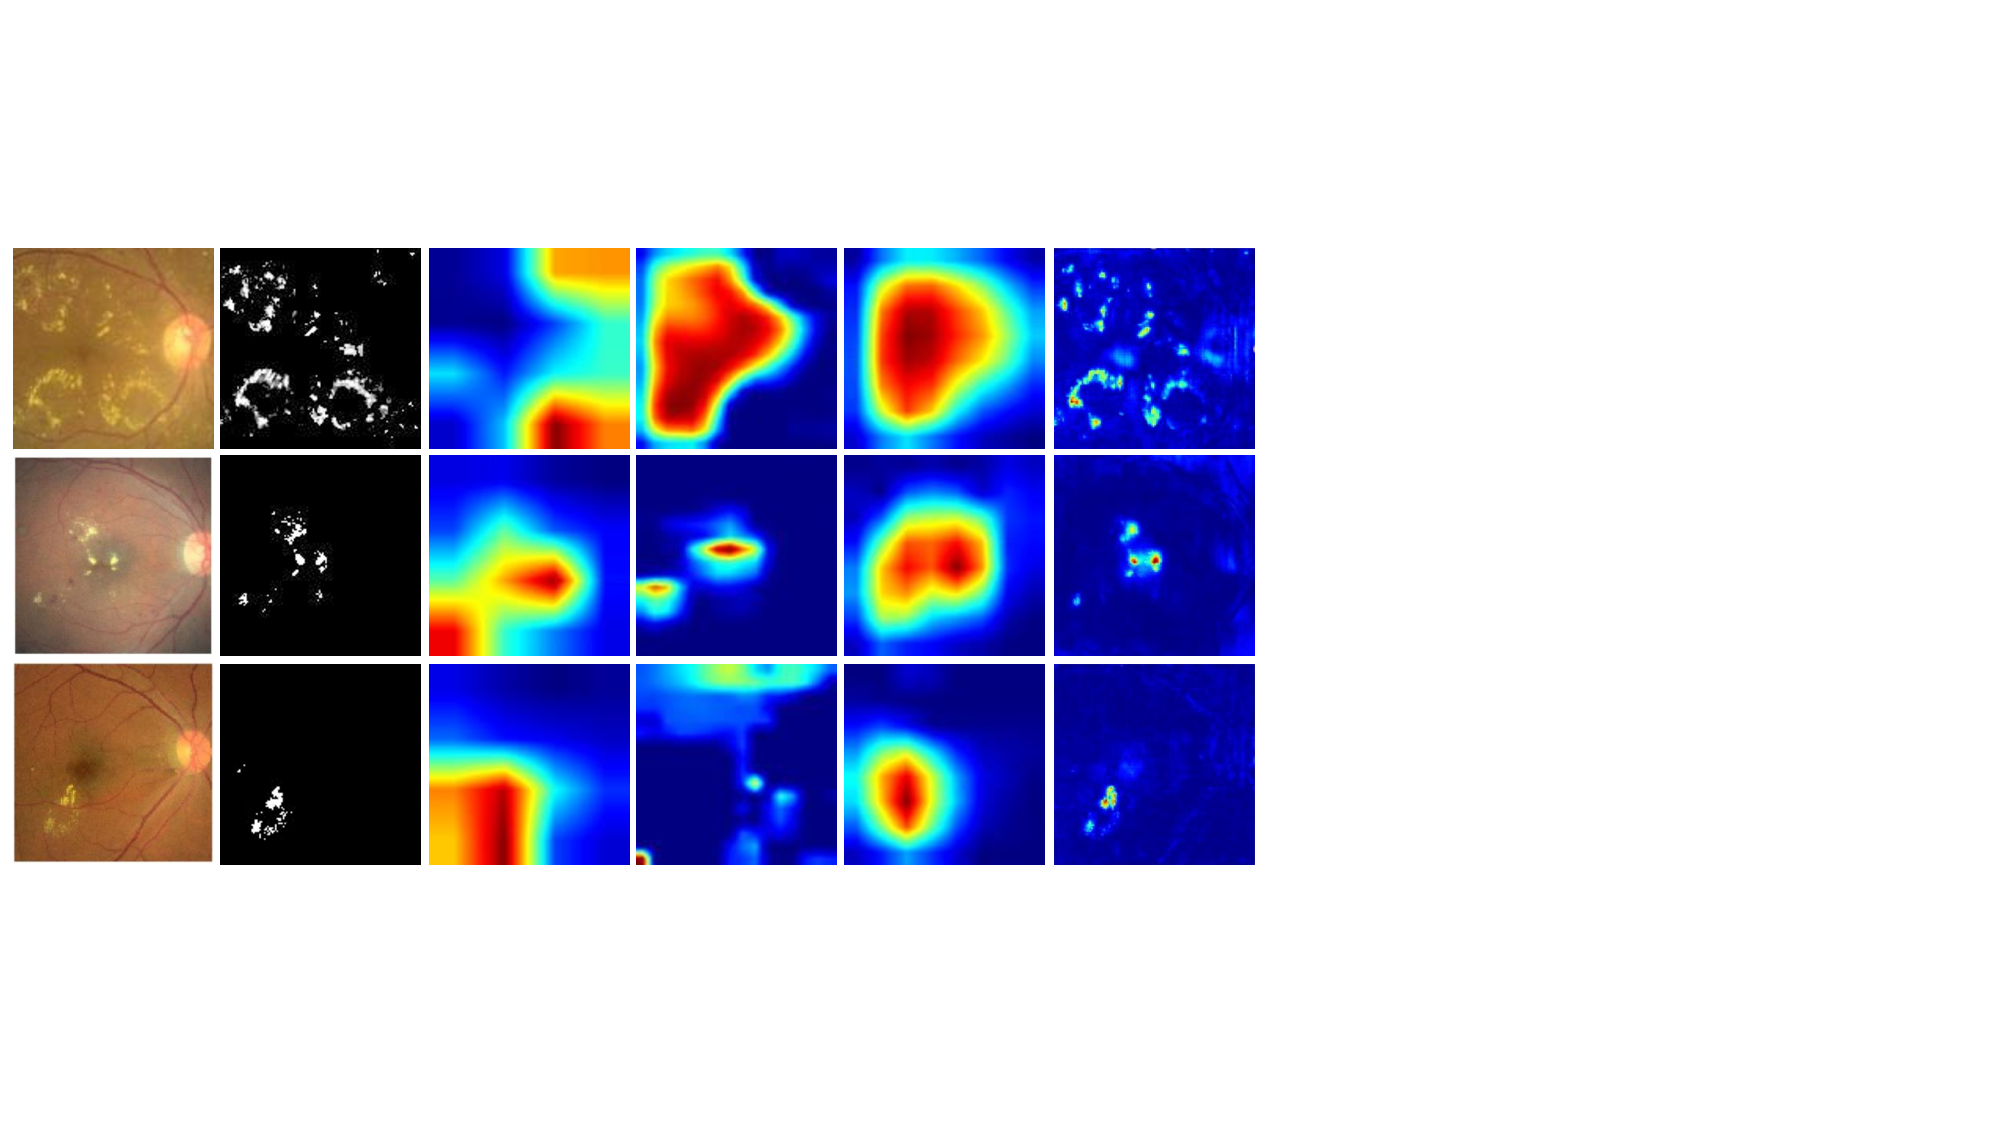
\includegraphics[width=1.0\textwidth]{figure/retinal_image_res.pdf}
	\caption{在视网膜糖尿病病变数据集上生物标记物定位结果。图中第$1$列表示原始异常图像,第$2$列表示其像素级标注,第$3$列表示CAM的定位结果,第$4$列表示Grad-CAM使用分类器中间层的特征图可视化的定位结果,第$5$列表示Grad-CAM使用分类器最后一层特征图可视化的定位结果,第$6$列是本文提出模型的定位结果。第$3-6$列表示输入图像的定位结果的热图,图中某一区域颜色越红,表示该区域为生物标记物的可能性越高。蓝色表示的意义与红色相反,表示其所在区域是生物标记物的可能性越低。以上颜色代表的意义同样适用于下文所有热图。}
	\label{fig:retinal_image_res}
\end{figure}

\noindent 如图\ref{fig:retinal_image_res}所示,从图中第$3$列定位结果可以看出,虽然CAM发现的生物标记物或者说异常区域最多,但是CAM也将周边区域作为生物标记物的一部分。这主要是由于将最后一个卷积层($4\times 4$)的输出向上采样到图像大小($128\times 128$)。另外,CAM也未能检测到第一幅图像(第$3$列,第$1$行)中的大部分异常区域。Grad-CAM作为CAM的扩展,它允许我们从多个层生成可视化的解释,例如中间卷积层(第$4$列,可记为Grad-CAM-1)和最后卷积层(第$5$列,可记为Grad-CAM-2)。虽然Grad-CAM-1在第$4$列(第三幅图像)获得了较为准确的生物标记物定位结果,但通过也将正常区域(图像中中间上方区域和左下角区域)误认作包含生物标记物的异常区域。更多的是其结果要么不够精确(第$1$行),要么不够精确(第$2$行和第$3$行)。与CAM相比,Grad-CAM-1实现了更为精确的定位结果,证明了其优于CAM的性能。另外,同样是由于对可视化特征图悬殊的上采样倍数($4\times 4 \rightarrow 128\times 128$),可以发现,Grad-CAM-2(第$5$列)标记的区域和CAM(第$3$列)没有太大区别。相比直线,本文提出的方法对形状不规则、分布分散的生物标记物进行了更精确的局部化(第$6$列),从定性分析的角度证明了其优于CAM和Grad-CAM的性能。

\begin{figure}[h]
	\centering
	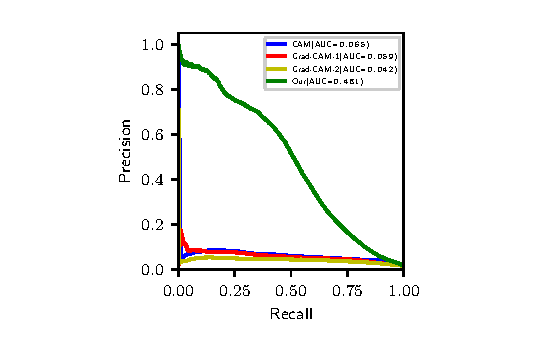
\includegraphics[width=1.0\textwidth]{figure/pr_curve_retinal_image/pr_curve.eps}
	\caption{CAM、Grad-CAM-1、本文提出的模型和Grad-CAM-2在40张视网膜糖尿病病变图像上画出的P-R曲线及其各自曲线下的面积(AUC,见右上角图例)。} 
	\label{fig:retinal_image_pr_curve}
\end{figure}

另外,本文充分利用二类视网膜糖尿病病变数据集中的$40$张像素级标注,通过对每种方法的定量评价,本文提出的模型、CAM、Grad-CAM-1和Grad-CAM-2的P-R曲线如图\ref{fig:retinal_image_pr_curve}所示。可以发现,绿色P-R曲线在其他三条曲线的上方,且与下侧横轴和左侧纵轴围成的封闭区域面积显然最大。以上四种方法各自对应的P-R曲线下的面积(AUC)分别为$0.481$,$0.065$,$0.061$和$0.042$,从而进一步从定量分析的角度证明了本文提出的模型在二类视网膜糖尿病病变数据集上的性能优越性。

\section{在二类模拟皮肤病病变数据集上的实验结果分析}\label{sec:bin_simulated_ds_experiment}
本节将展示本文提出的模型在模拟皮肤病病变数据集上的实验结果分析,本文提出的模型的比较对象同样是与CAM和Grad-CAM共计两种用于卷积神经网络可视化的方法进行比较,分定量分析和定性分析两个角度展开,下面进行具体叙述。

与\ref{sec:bin_dr_ds_experiment}小节一样,在本实验中,依然将ResNet-18作为CAM和Grad-CAM可视化的目标CNN分类器,同样没有单独设置测试集,分类器最终CNN分类准确率均达到了$99.7\%$以上。类似的,由于Grad-CAM可对卷积神经网络的任意层输出特征进行可视化,故在此实验中,同样选择了中间层输出特征(见图\ref{fig:simulated_skin}第$4$列)和最后一层输出特征(见图\ref{fig:simulated_skin}第$4$列)进行可视化,从而定位生物标记物。
\begin{figure}[h]
	\centering
	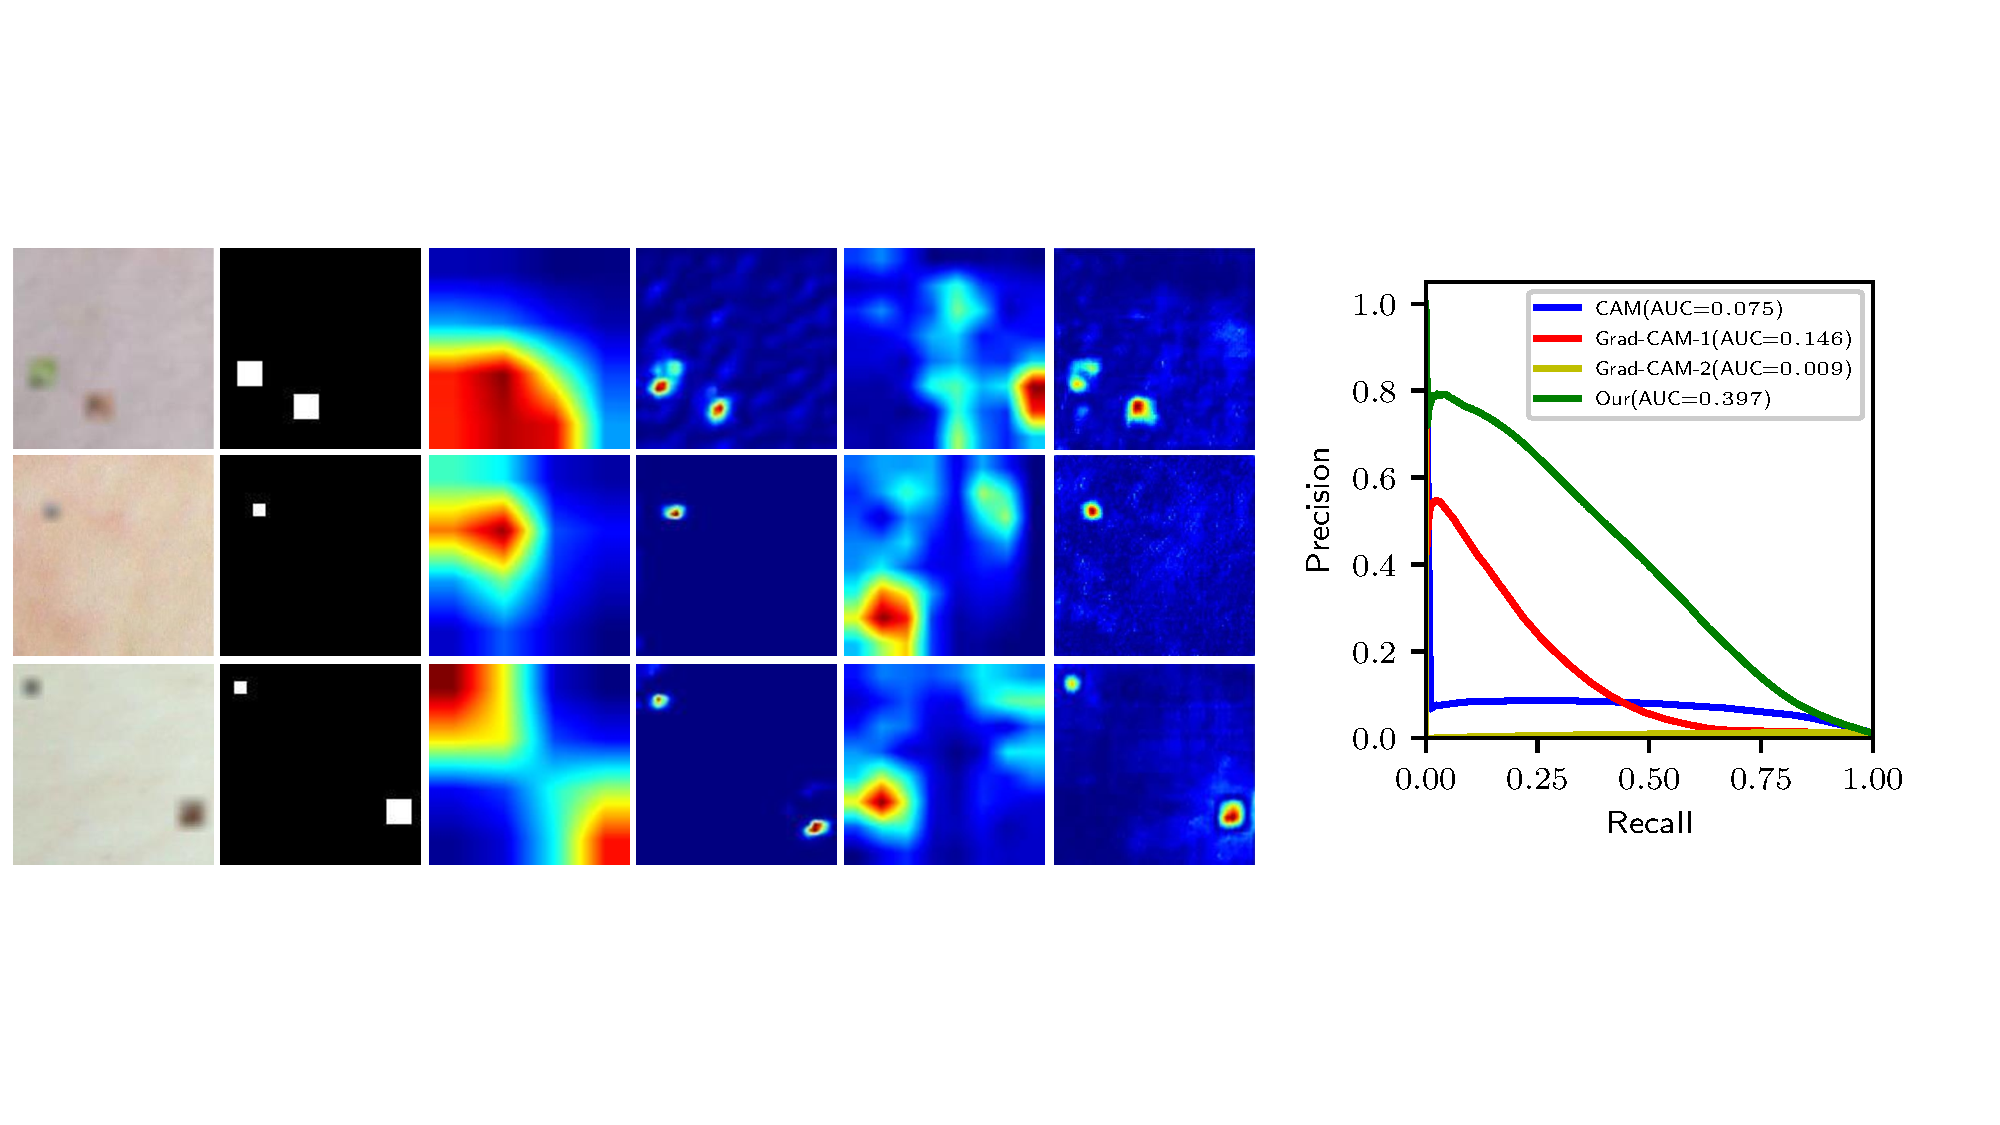
\includegraphics[width=1.0\textwidth]{figure/pr_curve_skin_image.pdf}
	\caption{在二类模拟皮肤病病变数据集上的生物标记物定位结果。图中第$1$列表示原始异常图像,第$2$列表示其像素级标注,第$3$列表示CAM的定位结果,第$4$列表示Grad-CAM使用分类器中间层的特征图可视化的定位结果(Grad-CAM-1),第$5$列表示Grad-CAM使用分类器最后一层特征图可视化的定位结果(Grad-CAM-2),第$6$列是本文提出模型的定位结果。} 
	\label{fig:simulated_skin}
\end{figure}

\noindent 从图\ref{fig:simulated_skin}可以看出,人工模拟生物标志物的皮肤图像进一步证实了本文提出的模型的优越性能。从图\ref{fig:simulated_skin}第$6$列可以看出,本文提出的方法几乎可以完美、精确地定位人工生物标记物,而CAM(第$3$列)和Grad-CAM(第$4$列和第$5$列)的性能再次表现出劣势。从总体上来说,第$4$列中生物标记物定位结果明显要比第$3$列更精确、更完美,也就能说明Grad-CAM在定位生物标记物上优于CAM。同样是由于特征图的过度上采样,CAM(第$3$列)和Grad-CAM-2(第$5$列)呈现类似的定位结果:虽然能检测到生物标记物的位置,但同时也包含了生物标记物周围的大量正常像素。之所以Grad-CAM-1(第$4$列)基本能精确定位到生物标记物的位置而极少包含生物标记物的周围像素,主要是因为Grad-CAM-1是通过对ResNet-18中第一个卷积层的特征输出的可视化结果来完成生物标记物的定位,其中上采样倍数较小($64\times 64\rightarrow 128\times 128$),这也能从侧面说明在该数据集上定位生物标记物要比在二类视网膜糖尿病病变数据集上容易得多(浅层特征便具备高级语义)。而CAM和Grad-CAM-2却都选择了最后一层卷积层的输出特征,其中上采样倍数要大得多($4\times4\rightarrow 128\times 128$)。

与CAM和Grad-CAM相比,图\ref{fig:simulated_skin}从定性分析的角度证明了本文提出的方法在二类模拟皮肤病病变数据集上的性能优越性,图\ref{fig:simulated_skin_pr_curve}再次从定性分析的角度证明了这一结论。CAM、Grad-CAM-1、Grad-CAM-2和本文提出的模型根据二类模拟皮肤病病变数据集上所有标注所得出的P-R曲线如图\ref{fig:simulated_skin_pr_curve}所示。不难看出,图中绿色曲线明显在其他三条曲线的上方,与下侧横轴和左侧纵轴围成的封闭区域的面积上,绿色曲线也明显大于其他三条曲线。以上四种方法各自对应的P-R曲线的AUC分别是$0.075$、$0.146$、$0.009$和$0.397$。
\begin{figure}[h]
	\centering
	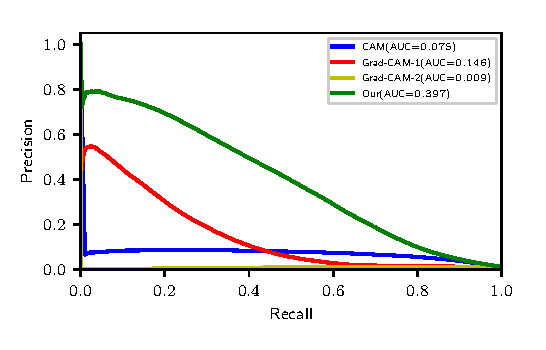
\includegraphics[width=1.0\textwidth]{figure/pr_curve_skin_image/pr_curve.eps}
	\caption{CAM、Grad-CAM-1、本文提出的模型和Grad-CAM-2在$1,310$张模拟皮肤病病变图像上画出的P-R曲线及其各自曲线下的面积(AUC,见右上角图例)。}
	\label{fig:simulated_skin_pr_curve}
\end{figure}

\section{CNN分类器和判别器角色探究}\label{sec:g_c_g_d_g_d_c_comparsion}
在\ref{sec:bin_dr_ds_experiment}小节和\ref{sec:bin_simulated_ds_experiment}小节中,本文通过定性分析和定量分析两个角度在二类视网膜糖尿病病变数据集和二类模拟皮肤病病变数据集上证明了本文提出的模型在生物标记物定位上的优越性能。为了进一步探究本文提出的模型中各个子模块在视网膜糖尿病病变图中扮演的角色以及添加的必要性(相关内容参见\ref{subsec:model_architecture}),本节内容将完成消融实验,分别去掉本文提出的模型中的CNN分类器和判别器,以探究CNN分类器模块和判别器模块的在整个模型中所起的作用。为了方便后续内容叙述,对于本文提出的模型,本文将其记为G-D-C模型,将移除判别器模块之后的模型记作编码器-解码器-CNN分类器(G-C)模型,将移除CNN分类器模块之后的模型记作编码器-解码器-判别器G-D模型。G-D-C模型、G-C模型和G-D模型的在二类视网膜糖尿病病变数据集上的部分实验结果如图\ref{fig:u_d_c_comparation}所示。
\begin{figure}[h]
	\centering
	\includegraphics[width=1.0\textwidth]{figure/u_d_c_comparation.pdf}
	\caption{G-D-C模型、G-C模型和G-D模型的在二类视网膜糖尿病病变数据集上的部分实验结果展示。第$1$列是原始输入图像,其中第一行是正常图像输入,第$2-4$行是异常图像输入。第$2$列是G-C模型的输出定位结果,第$3$列是第$2$列与第$1$列的差,第$4$列是G-D模型的输出定位结果,第$5$列是第$4$列与第$1$列的差,第$6$列是G-D-C模型给出的定位结果,第$7$列是第$6$列与第$1$列的差。第$4$列图像中的红色框表示其圈出部分的血管与原始输入图像相比发生了改变。} 
	\label{fig:u_d_c_comparation}
\end{figure}

从图\ref{fig:u_d_c_comparation}可以看出,当输入图像是正常图像时(图中第$1$行),G-D-C模型、G-C模型和G-D模型均能几乎不改变图像中的像素强度,只有在借助图中第$5$列和第$7$列的热图才能看出这张正常图像的左上角有些许改变。这说明对于正常图像,以上三种模型均能处理得比较好,以上三种模型的性能差异主要表现在处理异常图像(图中第$2-4$行)上。不难看出,在没有判别器的情况下(G-C模型),CNN分类器只能帮助定位了部分生物标记物(图中第$3$列热图),而将大部分生物标记物留在了编码器-解码器的输出(图中第$2$列)中。另一方面,在没有CNN分类器的情况下(G-D模型),判别器能定位到大部分(如果不是全部的话)的生物标记物区域(图中第$5$列)。然而,我们注意到,一些正常区域的像素强度同样也发生了改变(我们在第$4$列中用红色矩形框圈出),导致了一些正常的像素被错误得标记为生物标记物,包括一些包含血管的区域,这种发生改动的血管区域在第$5$列的热图中现实得更加突出。相比之下,编码器-解码器与CNN分类器以及判别器的组合(G-D-C模型)不仅可以精确定位大部分的生物标记物(图中第$7$列),在编码器-解码器的输出端(第$6$列)还能标记较少的假阳性生物标记物(图中第$7$列热图和第$5$列热图相比较)和更多的真实生物标记物(第$7$列热图和第$3$列热图相比较)。如\ref{sec:model_architecture_intro}小节描述,这些结果表明分类器和鉴别器网络共同帮助定位生物标志物。就各自角色而言,CNN分类器可在图像中定位生物标记物并在一定程度上帮助帮助编码器-解码器去除生物标记物(图中第$3$列),而判别器帮助编码器-解码器进一步去除CNN分类器未能定位或者未能去除的、难以去除的生物标记物。两者相辅相成(第$3$列与第$7$列比较),共同帮助编码器-解码器尽量去除图像中的所有生物标记物(图中第$7$列)。

\begin{figure}[h]
	\centering
	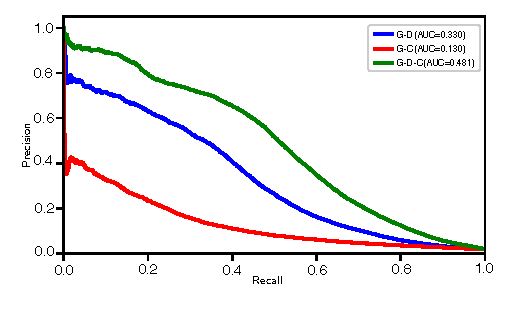
\includegraphics[width=1.0\textwidth]{figure/pr_cureve_u_d_u_c_u_d_c_components.pdf}
	\caption{G-D模型、G-C模型和G-D-C模型根据二类视网膜糖尿病病变数据集中标注的部分图像绘制的P-R曲线。三条曲线各自对应的AUC见右上角图例。} 
	\label{fig:u_d_c_comparation_pr_curve}
\end{figure}

为了对G-D模型、G-C模型和G-D-C模型进行更为精确的定量评价,本文再次使用二类视网膜糖尿病病变数据集中的$40$张像素级标注图像,进一步证实了以上结论。三者的P-C曲线如图\ref{fig:u_d_c_comparation_pr_curve}所示。可以发现,图中绿色的P-R曲线(G-D-C模型)在紫色(G-D模型)以及红色(G-C模型)P-R曲线上方,在曲线与左侧纵轴和下侧横轴围城的面积方面,绿色曲线显然围住了紫色以及红色P-R曲线,G-D-C模型(绿色曲线)、G-D模型(紫色曲线)和G-C模型(红色曲线)各自P-R曲线对应的AUC分别为$0.330$、$0.130$和$0.481$。这些现象再次表明G-D-C模型在视网膜糖尿病病变图像上的性能表现要优于G-D模型和G-C模型,同时也说明了CNN分类器和判别器的不可或缺行,符合\ref{subsec:model_architecture}小节中对二者的角色设计和期望。

另外,基于\ref{sec:idea_thinking}小节中的朴素思路,我们只使用正常图像训练编码器-解码器,希望编码器-解码器具有重建正常信号的能力,从而间接实现生物标记物的定位,本文将此素朴思路记为基准方法。然而,在二类视网膜糖尿病病变数据集上得到的AUC为$0.083$,远远低于G-C模型、G-D模型和G-D-C模型在此数据集上得到的结果(三者得到的AUC分别为为$0.130$、$0.330$和$0.481$),三者者均远远高于基准方法(更为直观的实验数据参见表\ref{tab:baseline_compared_diabetic_ds}),也能说明引入CNN分类器和判别器的必要性,从而再次佐证上述结论。
\begin{table}[h]
	\centering
	\caption{基准模型、G-C模型、G-D模型和G-D-C模型在二类视网膜糖尿病病变数据集上的实验结果表。表格展示的是通过P-R曲线计算的AUC分数。}		
	\label{tab:baseline_compared_diabetic_ds}
	\begin{tabular}{c|c|c|c|c}
		\toprule[2pt]
		模型名称 & 基准模型 & G-C模型 &G-D模型&G-D-C模型 \\
		\midrule[2pt]
		AUC	& $0.083$&	$0.130$ & $0.330$ & $0.481$	 \\
		\bottomrule[2pt]
	\end{tabular}
\end{table}

\section{对于经过编码器-解码器的视网膜糖尿病病变图像的定量分析}\label{sec:indirect_quantitative_evaluation}
在\ref{sec:bin_dr_ds_experiment}小节和\ref{sec:bin_simulated_ds_experiment}小节中,本文在二类模拟皮肤病病变数据集和二类视网膜病变数据集上利用已有的数据像素级标注进行了定量分析,这方式可看做是一种直接验证的方式。在本节中,本文将从间接角度来再次验证本文提出的模型在处理生物标记物定位问题的有效性。直观的想法是,在理想情况下,如果一种方法可以准确地定位和去除图像中的生物标记,则去除检测到的生物标记后的图像将不再包含生物标记物,那么去除检测到的生物标记后的图像将很难与原来的正常图像区分开来。基于以上想法,本文将二类视网膜糖尿病病变数据集按照$80$\%和$20$\%的比例分为训练集和验证集,为下文叙述方便,下文简称该数据集为“原始数据集”,并用训练集数据训练一个ResNet-18二类分类器。随后,对于训练集和验证集,每个图像都被输入到训练之后的编码器-解码器中,所有编码器-解码器的输出图像被收集起来,从而得到一个新的数据集,为了后文叙述方便,本文将该数据集记为“正常”数据集。最后,本文使用原始数据集训练得到的ResNet-18二类分类器对“正常”数据集分类。在此,本文使用Recall和Specificity作为分类器的评价标注。相关实验结果如表\ref{tab:quantitative_retinal}所示。

\begin{table}[h!]
	\begin{center}
		\caption{原始二类视网膜糖尿病病变数据集和“正常”数据集在ResNet-18分类器上的分类结果。前两列表示在原始数据集上的实验结果,后两列表示“正常”数据集上的实验结果。} 
		\label{tab:quantitative_retinal}
		\begin{tabular}{c|cc|cc}
			\toprule[2pt]
			& \multicolumn{2}{c|}{原始数据集} & \multicolumn{2}{c}{“正常”数据集} \\
			&  训练集 & 验证集 & 训练集 & 验证集\\
			\midrule[2pt]
			Recall & $0.958$ & $0.936$ & $0.269$ & $0.292$\\ \hline
			Specificity & $0.984$ & $0.964$ & $0.980$ & $0.964$\\
			\bottomrule[2pt]
		\end{tabular} 
	\end{center}
\end{table}

\noindent 从表\ref{tab:quantitative_retinal}不难看出,对于原始数据集(见表中前两列),ResNet-18分类器不仅在训练集上取得了较高的特异性(Specificity=$0.984$)和召回率(Recall=$0.958$),在测试集上也表现了优异性能(Recall和Specificity分别为$0.936$和$0.964$),说明ResNet-18分类器已经学会了寻找用于分类预测的生物标记物的特征。另外,表\ref{tab:quantitative_retinal}中后两列显示,大多数“正常”数据集中的异常图像在训练集和验证集上都被错误地归类为正常,导致更低的召回率(训练集和验证集上的Recall分别为$0.269$和$0.292$),说明本文提出的模型能够很好地定位并去除原始异常图像中的生物标记物,使得ResNet-18二分类器无法将去除生物标记物的图像与原始正常图像区分开来。另一方面,ResNet-18分类器在正常图像上具有较高的特异性值(训练集和验证集上分别为$0.980$和$0.964$),说明经过编码器-解码器后的正常图像仍然被正确分类为正常图像,这证实了编码器-解码器不会改变正常输入,也从实验角度证明了在\ref{ite:ideal_situation}小节中提出的设想。总之,在原始数据集和“正常”数据集上,无论对于其中的训练集还是验证集,召回率的大幅下降和特异性的小幅下降表明,本文提出的模型可以很好地从图像中去除潜在的生物标记物,同时保持正常区域不变。从而再次从CNN分类器的角度证明了本文提出的方法的优异性能。
\begin{figure}[h]
	\centering
	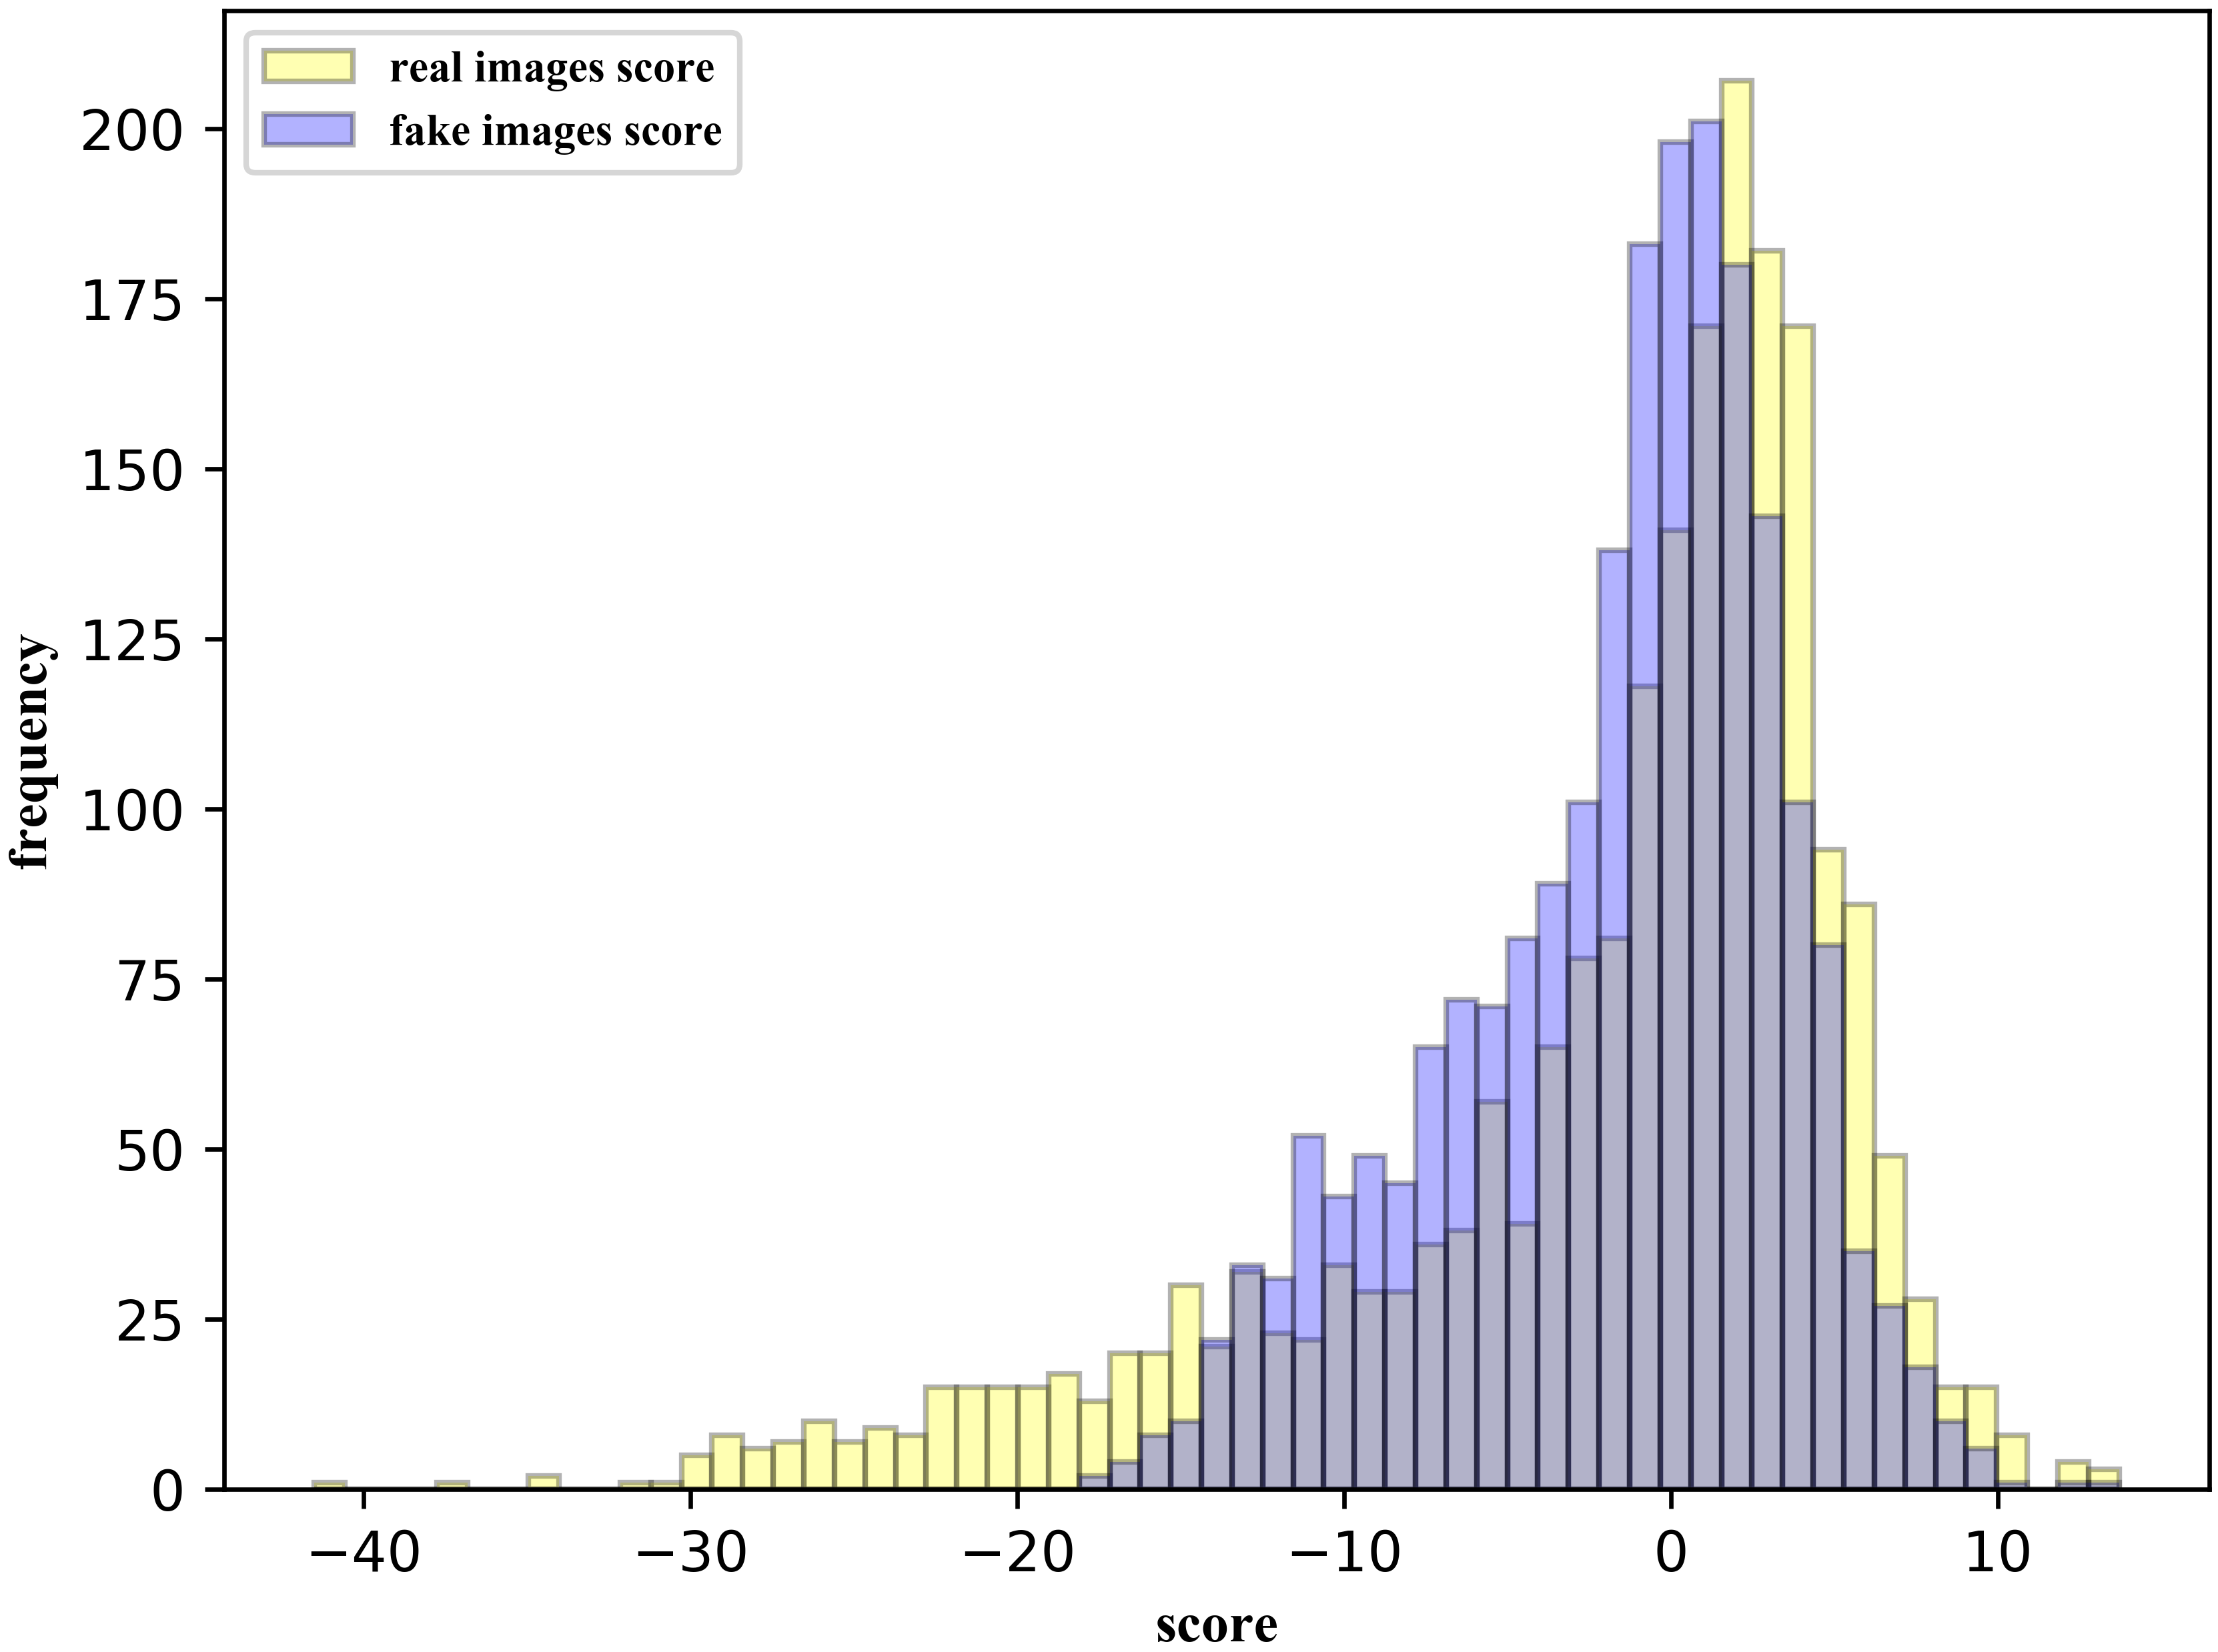
\includegraphics[width=1.0\textwidth]{figure/score_distribution.png}
	\caption{将原始数据集中的正常图像和“正常”数据集中的“正常”图像分别送入到判别器之后,根据输出分数绘制的频率分布直方图。黄色柱子表示判别器真图像输入端的输出分数,紫色柱子表示判别器假图像输入端的输出分数,灰色柱子表示以上两者的重叠部分。}
	\label{fig:hist_freq}
\end{figure}

\noindent 另外,训练结束后,我们还将“正常”数据集中的正常图像和异常图像均送入判别器,判别器输出分数的频率分布直方图如图\ref{fig:hist_freq}所示。不难从直方图中看出,送入判别器的两端分数的频率分布直方图有较大重叠部分,如果暂时不考虑原始图像中的离群点(直方图中靠近下侧横轴最左端的分数),则两者分解输出分数会更加接近。我们还可以根据以上直方图可计算得到,判别器对于“正常”数据集中的正常图像和异常图像输出的平均输出分数分别为$-2.1$和$-1.7$,而在初始参数下,两者的平均分数分别为$-2.2$和$-1.0$,这说明训练结束后,判别器输出端的图像相似度得到极大提升(判别器两端输出平均分数的差值大大缩小:$1.2\rightarrow 0.4$)。总之,以上现象可说明,对于正常图像输入,编码器-解码器基本不改变其像素强度;而对于异常图像输入,经过编码器-解码器的输出与不断向正常图像输出靠近,也从判别器的角度间接说明编码器-解码能够比较好地去除原始数据集中的生物标记物。

\section{不同超参数下的实验结果分析}\label{sec:hyper_paras}
为了验证本文提出的模型的超参数鲁棒性(损失函数见等式\ref{equ:model_loss_func}),本文对损失函数中的两个超参数$\lambda_{1}$和$\lambda_{2}$进行测试,旨在找出比较鲁邦的超参数范围。为此,在保证学习率、迭代次数、网络参数初始化等所有相关设置相同的情况下,本文取了$6$种不同的$\lambda_{1}$和$\lambda_{2}$超参数取值,在二类糖尿病病变数据进行了相关测试。这里同样使用P-R曲线及其AUC分数作为评价标准。相关实验结果如图\ref{fig:pr_curve_retinal_hyper_paras}所示。

\begin{figure}[h]
	\centering
	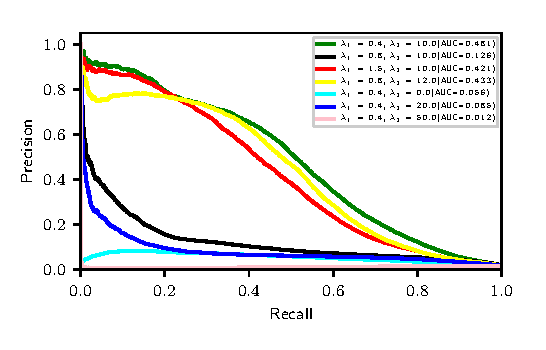
\includegraphics[width=1.0\textwidth]{figure/pr_curve_retinal_hyper_paras/pr_curve.eps}
	\caption{不同超参数$\lambda_{1}$和$\lambda_{2}$组合下,本文提出的模型在二类糖尿病病变数据上得到的P-R曲线及其AUC(见右上角图例)。} 
	\label{fig:pr_curve_retinal_hyper_paras}
\end{figure}

从图\ref{fig:pr_curve_retinal_hyper_paras}可以看出,在$\lambda_{1}=0.4, \lambda_{2}=10$、$\lambda_{1}=1.5,\lambda_{2}=10$和$\lambda_{1}=0.8,\lambda_{2}=12$这三组超参数设置下,模型性能表现比较稳定,AUC取值分别为$0.481$(图中绿色曲线)、$0.421$(图中红色曲线)和$0.433$(图中黄色曲线)。说明$\lambda_{1}\in [0.4,1.5]$,$\lambda_{2}\in [10,12]$范围内,文本提出的模型的性能比较稳定。另外,注意到$\lambda_{1}=0.4,\lambda_{2}=0$时,本文模型取得较低AUC($0.056$,图中青色曲线),说明损失函数中L1损失对编码器-解码器输入输出约束的必要性(见等式~\ref{equ:model_loss_func})。而当$\lambda_{2}\geq 20$时,本文提出模型的性能也比较差,其中,$\lambda_{2}=20$时,AUC为$0.085$(图中蓝色曲线);$\lambda_{2}=50$时,AUC为$0.012$(图中品红色曲线),这主要是因为当$\lambda_{2}$过大时,在损失函数中真正起主导作用的是L1损失函数,此时,无论对于异常图像还是正常图像输入,编码器-解码器模块的输入输出均变化不大,从而导致生物标记物定位失败,表现出AUC较低,比较接近基准模型(相关叙述见\ref{sec:g_c_g_d_g_d_c_comparsion}小节)的定位性能。而另一个极端,当$\lambda_{1}\rightarrow 0$时,相当于模型中移去CNN分类器,相关结果在\ref{sec:g_c_g_d_g_d_c_comparsion}小节中已有展示。另外,为了更为直观的观察不同超参取值下的模型性能,本文将超参数组合与对应AUC分数列在表\ref{tab:diff_parameters}中。

\begin{table}[h]
	\centering
	\caption{不同超参数组合下,本文提出的模型在二类视网膜糖尿病病变数据集上计算得到的AUC分数列表。}		
	\label{tab:diff_parameters}
	\resizebox{1.0\textwidth}{!}{
		\begin{tabular}{c|c|c|c|c|c|c}
			\toprule[2pt]
			 & $\lambda_{1}=0.4,\lambda_{2}=10)$ & $(0.8, 10)$& $\lambda_{1}=1.5, \lambda_{2}=10)$&
			$\lambda_{1}=0.4,\lambda_{2}=0$& $\lambda_{1}=0.4,\lambda_{2}=20$ & $\lambda_{1}=0.4,\lambda_{2}=50$ \\
			\midrule[2pt]
			AUC	& $0.481$ &	$0.421 $ & $0.433$ & $0.056$ & $0.085$& $0.012$	 \\
			\bottomrule[2pt]
		\end{tabular}
	}
\end{table}
\section{对判别器模型结构的探究}\label{sec:dis_arch}
本文

另外,
\section{本章小结}
本章主要展示了在二类模拟皮肤病病变数据集和二类视网膜糖尿病病变数据集上的相关实验结果及其分析,与CAM和Grad-CAM,在评价标准P-R曲线及其AUC方面,本文提出的模型可以实现更为精确的生物标记物定位结果。另外,为了让读者更清楚理解本文提出的模型的内部情况,本章设计了系列消融实验,例如在\ref{sec:g_c_g_d_g_d_c_comparsion}小节中通过分别去掉CNN分类器和判别器的方式来探究二者在完整模型中所起到的作用。除了直接与CAM和Grad-CAM作比较来证明本文提出的模型的性能优越性,还通过间接方式分别从CNN分类器和判别器进行了进一步验证(参加\ref{sec:indirect_quantitative_evaluation}小节)。最后,还分别设计了两组对比实验分别探究了本文提出的模型的适用超参数范围和判别器结构变化对于整体模型的影响。到此,本文提出的模型在二类生物标记物的精确定位问题叙述完毕,接下来将在第\ref{sec:multi_classes}章中展示本文提出的模型在处理多类生物标记物的精确定位问题的相关实验结果。如\ref{sec:existing_diffcuities}小节中所描述的那样,由二分类生物标记物的定位问题到多分类生物标记物的定位问题并不是一个简单的二类到多类的推广,而是存在诸多难题。在数据集方面,图像数量比较多、图像质量比较高的多类数据集难以收集,而且图像的像素级标注代价高昂的问题依然存在。在模型的训练方面,对于CNN分类器的处理比较容易,将二类交叉熵损失替换成多类交叉熵即可,难点是如何处理判别器,因为对抗生成网络只有正常/异常两个输入端,是否要添加新的判别器来处理新加入的类别,另外,存在多个类别时,如何组织数据训练模型,这些均是值得考虑的问题。接下来,在第\ref{sec:multi_classes}章中,本文将针对以上问题展开相关内容的叙述,同时选取可用于多类生物标记物精确定位任务相关的数据集,最后展示相关实验结果并对其进行分析。


